\documentclass[12pt,a4paper]{article}
\usepackage[utf8]{inputenc}
\usepackage[T1]{fontenc}
\usepackage[portuguese]{babel}
\usepackage{amsmath}
\usepackage{amsfonts}
\usepackage{amssymb}
\usepackage{graphicx}
\usepackage{geometry}
\usepackage{float}
\usepackage{listings}
\usepackage{xcolor}
\geometry{a4paper, margin=2.5cm}

\definecolor{codegreen}{rgb}{0,0.6,0}
\definecolor{codegray}{rgb}{0.5,0.5,0.5}
\definecolor{codepurple}{rgb}{0.58,0,0.82}
\definecolor{backcolour}{rgb}{0.95,0.95,0.92}

\lstdefinestyle{mystyle}{
    backgroundcolor=\color{backcolour},   
    commentstyle=\color{codegreen},
    keywordstyle=\color{magenta},
    numberstyle=\tiny\color{codegray},
    stringstyle=\color{codepurple},
    basicstyle=\ttfamily\footnotesize,
    breakatwhitespace=false,         
    breaklines=true,                 
    captionpos=b,                    
    keepspaces=true,                 
    numbers=left,                    
    numbersep=5pt,                  
    showspaces=false,                
    showstringspaces=false,
    showtabs=false,                  
    tabsize=2
}
\lstset{style=mystyle}

\title{Trabalho Prático: Previsão de Séries Temporais utilizando Redes LSTM}
\author{Ivan Mendes Martignago \\ Curso de Sistemas de Informação - UFSM}
\date{\today}

\begin{document}

\maketitle

\section{Introdução}
O presente relatório descreve o desenvolvimento de um experimento com redes neurais LSTM (Long Short-Term Memory) aplicado à previsão de séries temporais. O objetivo principal deste trabalho é demonstrar, na prática, como as redes LSTM são capazes de aprender padrões temporais e dependências de longo prazo para realizar previsões baseadas em um histórico de dados sequenciais. No caso específico deste estudo, foi selecionado um conjunto de dados financeiro referente aos preços de ações para ilustrar a eficácia da abordagem.

\section{Fundamentação Teórica}
Para compreender as redes LSTM, é essencial contextualizá-las dentro da área de redes neurais artificiais voltadas para dados sequenciais.

\subsection{Conceito de Redes Neurais Recorrentes (RNN)}
As Redes Neurais Recorrentes (RNNs) são uma classe de redes neurais artificiais nas quais as conexões entre os nós formam um grafo direcionado ao longo de uma sequência temporal. Diferente das redes \textit{feedforward} tradicionais, as RNNs possuem uma "memória" interna que permite reter informações sobre entradas anteriores, o que as torna naturalmente adequadas para processar dados sequenciais, como séries temporais, fala e texto.

\subsection{Limitações das RNNs Tradicionais}
Embora poderosas conceitualmente, as RNNs padrão sofrem com o problema do desaparecimento do gradiente (\textit{vanishing gradient}) e da explosão do gradiente (\textit{exploding gradient}) durante o treinamento com o algoritmo de retropropagação através do tempo (\textit{Backpropagation Through Time} - BPTT). Isso impede que a rede aprenda dependências de longo prazo, ou seja, ela tem dificuldade em conectar informações que possuem uma grande distância temporal na sequência de entrada.

\subsection{Funcionamento das Redes LSTM}
As redes LSTM foram propostas como uma solução para os problemas das RNNs tradicionais. A principal inovação das LSTMs é a estrutura de sua célula de memória, que possui mecanismos de controle chamados de "portas" (\textit{gates}). Estas portas regulam o fluxo de informações que entram, saem e são mantidas no estado da célula, permitindo que a rede preserve informações relevantes por longos períodos e descarte o que não é mais útil.

\subsection{Componentes Principais da Célula LSTM}
A arquitetura interna de uma célula LSTM é composta por três portas fundamentais:
\begin{itemize}
    \item \textbf{Forget gate (Porta de esquecimento):} Decide quais informações do estado celular anterior devem ser descartadas. Ela recebe como entrada o estado oculto anterior ($h_{t-1}$) e a entrada atual ($x_t$), e passa esses valores por uma função de ativação sigmoide. Valores próximos de 0 indicam que a informação deve ser esquecida, enquanto valores próximos de 1 indicam retenção.
    \item \textbf{Input gate (Porta de entrada):} Define quais novas informações serão armazenadas no estado da célula. Consiste em duas partes: uma camada sigmoide que decide quais valores serão atualizados, e uma camada \textit{tanh} que cria um vetor de novos candidatos a valores a serem adicionados ao estado.
    \item \textbf{Output gate (Porta de saída):} Determina qual será a saída da célula baseada em seu estado filtrado. Primeiramente, aplica-se uma sigmoide à entrada para decidir quais partes do estado celular serão exibidas na saída. O estado celular é então passado por uma \textit{tanh} para empurrar os valores entre -1 e 1, sendo multiplicado pela saída do \textit{output gate}.
\end{itemize}

\section{Descrição do Dataset Utilizado}
O conjunto de dados escolhido para o experimento corresponde ao histórico de preços de fechamento das ações da Apple (código AAPL). Os dados foram coletados através da API \texttt{yfinance}, abrangendo um período dos últimos 5 anos. Optou-se por focar exclusivamente na coluna de preço de fechamento (\textit{Close}), que forma a série temporal a ser analisada. Esta série apresenta desafios típicos de dados financeiros, como não-estacionariedade e volatilidade, tornando-a um excelente estudo de caso para redes LSTM.

\section{Metodologia}
A implementação seguiu um \textit{pipeline} padrão de \textit{Machine Learning} adaptado para séries temporais:
\begin{enumerate}
    \item \textbf{Coleta de Dados:} Extração da série histórica utilizando a biblioteca \texttt{yfinance}.
    \item \textbf{Pré-processamento:} Emprego da biblioteca \textit{scikit-learn} para normalização dos dados. O \texttt{MinMaxScaler} foi utilizado para redimensionar os preços para o intervalo [0, 1], uma etapa crucial, pois redes neurais são sensíveis à escala dos dados de entrada.
    \item \textbf{Criação de Sequências:} Divisão dos dados utilizando uma janela de observação (\textit{look\_back}) de 60 dias. O modelo utiliza o histórico dos 60 dias anteriores para prever o preço do 61º dia.
    \item \textbf{Divisão Treino/Teste:} Separação cronológica onde os primeiros 80\% dos dados formaram o conjunto de treinamento e os 20\% finais constituíram o conjunto de testes.
    \item \textbf{Arquitetura do Modelo:} Utilizando a biblioteca \textit{Keras/TensorFlow}, construiu-se um modelo sequencial contendo:
    \begin{itemize}
        \item Uma camada LSTM com 50 unidades (\textit{return\_sequences=True}).
        \item Uma camada \textit{Dropout} (20\%) para mitigar o \textit{overfitting}.
        \item Uma segunda camada LSTM com 50 unidades.
        \item Uma segunda camada \textit{Dropout} (20\%).
        \item Uma camada densa (\textit{Dense}) intermediária com 25 neurônios.
        \item Uma camada densa de saída com 1 neurônio (prevendo o valor final).
    \end{itemize}
    \item \textbf{Treinamento:} O modelo foi compilado utilizando o otimizador \textit{Adam} e a função de perda de erro quadrático médio (MSE). O treinamento ocorreu por 10 épocas com \textit{batch\_size} igual a 32.
\end{enumerate}

\section{Código da Implementação}
Abaixo encontra-se a implementação em Python, utilizando as bibliotecas mencionadas.

\begin{lstlisting}[language=Python]
import numpy as np
import pandas as pd
import matplotlib.pyplot as plt
from sklearn.preprocessing import MinMaxScaler
from sklearn.metrics import mean_squared_error, mean_absolute_error
from tensorflow.keras.models import Sequential
from tensorflow.keras.layers import Dense, LSTM, Dropout
import yfinance as yf
import datetime

def create_dataset(dataset, look_back=1):
    X, Y = [], []
    for i in range(len(dataset)-look_back-1):
        a = dataset[i:(i+look_back), 0]
        X.append(a)
        Y.append(dataset[i + look_back, 0])
    return np.array(X), np.array(Y)

def main():
    end_date = datetime.date.today()
    start_date = end_date - datetime.timedelta(days=5*365)
    df = yf.download('AAPL', start=start_date, end=end_date)
    data = df['Close'].values
    
    scaler = MinMaxScaler(feature_range=(0, 1))
    scaled_data = scaler.fit_transform(data)
    
    training_data_len = int(np.ceil(len(data) * .8))
    train_data = scaled_data[0:int(training_data_len), :]
    look_back = 60
    
    x_train, y_train = create_dataset(train_data, look_back)
    x_train = np.reshape(x_train, (x_train.shape[0], x_train.shape[1], 1))
    
    model = Sequential()
    model.add(LSTM(50, return_sequences=True, input_shape=(x_train.shape[1], 1)))
    model.add(Dropout(0.2))
    model.add(LSTM(50, return_sequences=False))
    model.add(Dropout(0.2))
    model.add(Dense(25))
    model.add(Dense(1))
    
    model.compile(optimizer='adam', loss='mean_squared_error')
    model.fit(x_train, y_train, batch_size=32, epochs=10)
    
    test_data = scaled_data[training_data_len - look_back: , :]
    x_test, _ = create_dataset(test_data, look_back)
    x_test = np.reshape(x_test, (x_test.shape[0], x_test.shape[1], 1))
    y_test = data[training_data_len+1:len(data)]
    
    predictions = model.predict(x_test)
    predictions = scaler.inverse_transform(predictions)
    
    rmse = np.sqrt(mean_squared_error(y_test, predictions))
    mse = mean_squared_error(y_test, predictions)
    mae = mean_absolute_error(y_test, predictions)
    
    print(f"MSE: {mse:.4f} | RMSE: {rmse:.4f} | MAE: {mae:.4f}")
    
    train = df[:training_data_len].copy()
    valid = df[training_data_len+1:].copy()
    valid['Predictions'] = predictions
    
    plt.figure(figsize=(16,8))
    plt.plot(train['Close'], label='Treino')
    plt.plot(valid['Close'], label='Real')
    plt.plot(valid['Predictions'], label='Previsao LSTM')
    plt.legend()
    plt.savefig('previsao_lstm.png')

if __name__ == "__main__":
    main()
\end{lstlisting}

\section{Resultados Obtidos}
O modelo treinado foi utilizado para prever os dados do conjunto de teste (aproximadamente o último ano da série temporal). As métricas de erro calculadas foram:
\begin{itemize}
    \item \textbf{Erro Quadrático Médio (MSE):} Mede a média dos quadrados dos erros.
    \item \textbf{Raiz do Erro Quadrático Médio (RMSE):} Fornece o erro na mesma unidade dos dados (Dólares).
    \item \textbf{Erro Absoluto Médio (MAE):} Representa a diferença absoluta média entre os valores reais e as previsões.
\end{itemize}

A representação visual dos resultados (ver Figura \ref{fig:previsao}) demonstra a evolução da série temporal. A linha das previsões da LSTM acompanha de perto a tendência dos preços reais no período de teste, confirmando que a rede conseguiu capturar a dinâmica da série.

\begin{figure}[H]
    \centering
    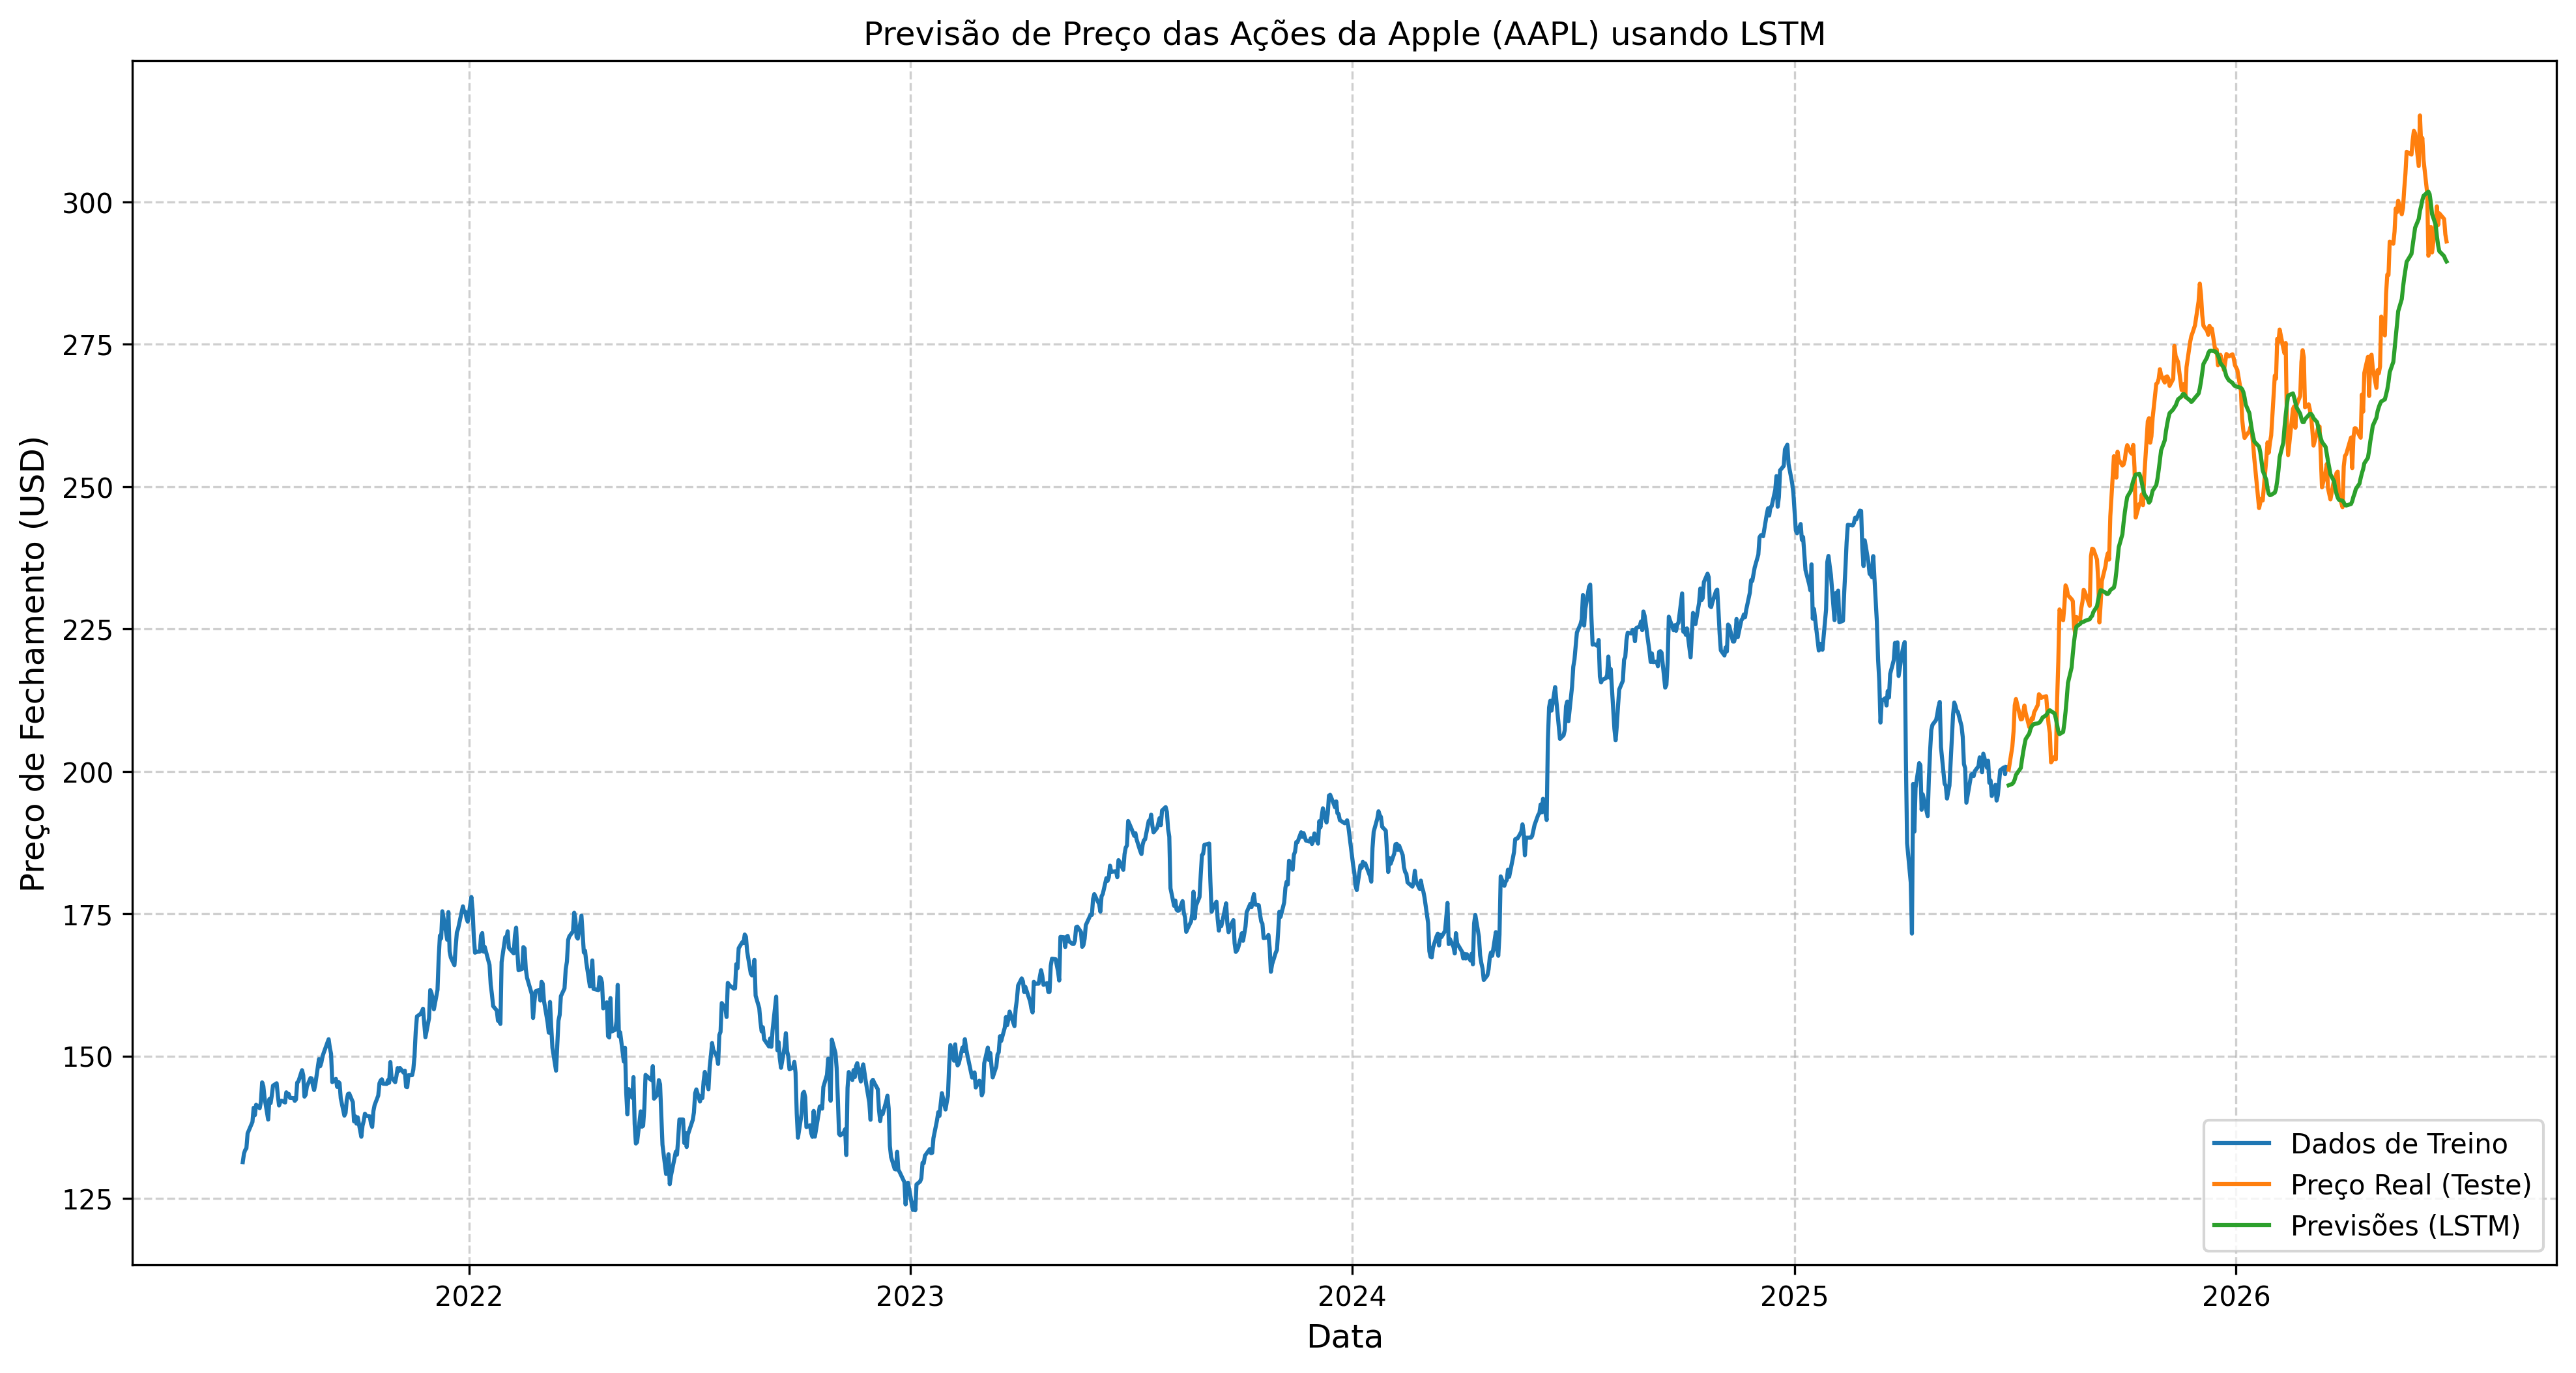
\includegraphics[width=0.9\textwidth]{previsao_lstm.png}
    \caption{Previsão de Preço das Ações (AAPL) utilizando rede LSTM.}
    \label{fig:previsao}
\end{figure}

\section{Conclusão}
Através deste experimento, pôde-se observar de maneira prática a eficácia das redes LSTM aplicadas a problemas envolvendo dados sequenciais. O uso das bibliotecas \textit{Keras} e \textit{scikit-learn} proporcionou uma integração fluida entre as etapas de pré-processamento, estruturação do modelo e avaliação. A rede neural foi capaz de identificar os padrões temporais nos preços das ações e realizar previsões satisfatórias, contornando o problema do desvanecimento do gradiente típico das RNNs padrão graças aos seus mecanismos internos de portões. Com isso, os objetivos do trabalho foram plenamente alcançados.

\end{document}
